\documentclass[12pt,a4paper]{article}
\usepackage[utf8]{vietnam}
\usepackage{amsmath,amssymb}
\usepackage{tabularx}
\usepackage{tikz}
\usetikzlibrary{intersections}
\usepackage{xcolor}
\usepackage[top=0.6cm, bottom=0.6cm, left=0.6cm, right=0.6cm]{geometry}
\usepackage[dethi]{ex_test}

\setlength{\parskip}{0pt}

% Dòng kẻ chấm mờ đều đặn chuẩn viết tay (khoảng cách ~6.7mm chuẩn vở học sinh)
\newcommand{\dongke}[1]{%
  \begingroup%
  \setlength{\parskip}{0pt}%
  \baselineskip=19.0pt%
  \vspace{0.8mm}%
  \foreach \i in {1,...,#1}{%
    \noindent{\color{gray!60}\dotfill}\par%
  }%
  \vspace{0.6mm}%
  \endgroup%
}

% Định nghĩa ô bài tập tự luận trong bảng
\newcommand{\oBaiTap}[3][6]{%
  \vspace{0.8mm}%
  \noindent\textbf{#2} #3\par%
  \dongke{#1}%
}

% Câu trắc nghiệm 1 dòng: 4 đáp án dàn hàng ngang
\newcommand{\cauTN}[6]{% \cauTN{số câu}{đề}{A}{B}{C}{D}
  \noindent\textbf{Câu #1.} #2\par\vspace{0.4mm}%
  \noindent%
  \makebox[0.25\linewidth][l]{\textbf{A.} #3}%
  \makebox[0.25\linewidth][l]{\textbf{B.} #4}%
  \makebox[0.25\linewidth][l]{\textbf{C.} #5}%
  \makebox[0.25\linewidth][l]{\textbf{D.} #6}\par\vspace{1.0mm}%
}

% Khung Giả thiết - Kết luận dạng dấu cộng (GT góc II, KL góc III, để trống không dòng kẻ)
\newcommand{\oGTKL}{%
  \vspace{0.5mm}%
  \noindent\hfil%
  \begin{tikzpicture}[line join=round, line cap=round]
    % Đường ngang phân cách GT và KL
    \draw[thick] (0.1, 1.1) -- (9.1, 1.1);
    % Đường dọc phân cách cột nhãn và cột nội dung
    \draw[thick] (1.5, 0.1) -- (1.5, 2.7);
    % Nhãn GT (nằm chính giữa góc phần tư thứ 2)
    \node at (0.8, 1.9) {\textbf{\large GT}};
    % Nhãn KL (nằm chính giữa góc phần tư thứ 3)
    \node at (0.8, 0.6) {\textbf{\large KL}};
    % Bounding box vô hình
    \path (0, 0) rectangle (9.2, 2.8);
  \end{tikzpicture}\hfil\null\par%
  \vspace{0.5mm}%
}

\begin{document}
\pagestyle{empty}

% =============================================================================
% ========================= TOÁN 7 - TUẦN 05 - BUỔI 02: MÃ ĐỀ 101 =============
% ========================= MẶT TRƯỚC (TRANG 1/2) ==============================
% =============================================================================

\noindent
\begin{tabularx}{\linewidth}{|X|c|}
\hline
\textbf{PHIẾU KIỂM TRA ĐỊNH KỲ TOÁN 7 - TUẦN 05 - BUỔI 02} & \textbf{Mã đề: 101 - Trang 1/2} \\
\textit{Chủ đề: Tổng ôn tập Số hữu tỉ \& Hình học tính góc} & \textit{Thời gian: 45 phút} \\
\hline
\end{tabularx}

\vspace{0.8mm}

\noindent
\begin{tabularx}{\linewidth}{|X|}
\hline
\rule[-2mm]{0pt}{8mm}\textbf{Họ và tên học sinh:} \hfill \textbf{SĐT:} \makebox[4.5cm]{\dotfill} \\
\hline
\end{tabularx}

\vspace{0.8mm}

\noindent
\begin{tabularx}{\linewidth}{|p{3.2cm}|X|}
\hline
\centering\textbf{ĐIỂM SỐ} & \centering\textbf{LỜI NHẬN XÉT CỦA THẦY CÔ} \tabularnewline
\hline
\rule{0pt}{1.8cm} & \tabularnewline
\hline
\end{tabularx}

\vspace{1mm}

\noindent\textbf{\large PHẦN I. TRẮC NGHIỆM KHÁCH QUAN (2,5 điểm)} \hfill \textit{(Khoanh tròn đáp án đúng)}
\vspace{0.8mm}

\cauTN{1}{Làm tròn số thập phân $3{,}14159...$ đến hàng phần trăm ta được số:}{$3{,}15$}{$3{,}14$}{$3{,}142$}{$3{,}1$}

\cauTN{2}{Kết quả của phép tính lũy thừa $\left(-\dfrac{1}{2}\right)^3$ là:}{$-\dfrac{1}{8}$}{$\dfrac{1}{8}$}{$-\dfrac{1}{6}$}{$\dfrac{1}{6}$}

\cauTN{3}{Cho đẳng thức $x + \dfrac{1}{3} = \dfrac{4}{5}$. Theo quy tắc chuyển vế thì $x$ bằng:}{$\dfrac{4}{5} + \dfrac{1}{3}$}{$\dfrac{4}{5} - \dfrac{1}{3}$}{$-\dfrac{4}{5} - \dfrac{1}{3}$}{$\dfrac{1}{3} - \dfrac{4}{5}$}

\cauTN{4}{Nếu một đường thẳng cắt hai đường thẳng song song thì hai góc trong cùng phía:}{bằng nhau}{phụ nhau}{bù nhau}{kề bù}

\cauTN{5}{Cho hai đường thẳng phân biệt $a, b$ cùng vuông góc với đường thẳng $c$ thì:}{$a \perp b$}{$a \equiv b$}{$a$ cắt $b$}{$a \parallel b$}

\vspace{1mm}

\noindent\textbf{\large PHẦN II. TỰ LUẬN (7,5 điểm)}

\noindent\textbf{Câu 2 (2,5 điểm). Thực hiện phép tính (hợp lý nếu có thể):}
\vspace{0.5mm}

\noindent
\begin{tabularx}{\linewidth}{|X|X|}
\hline
\oBaiTap[8]{a)}{$\dfrac{3}{5} - \dfrac{5}{6} + \dfrac{7}{10}$} & 
\oBaiTap[8]{b)}{$\dfrac{7}{15} \cdot \left(-\dfrac{3}{8}\right) + \dfrac{7}{15} \cdot \left(-\dfrac{5}{8}\right)$} \\
\hline
\oBaiTap[8]{c)}{$\left(-\dfrac{1}{2}\right)^2 + \dfrac{3}{4} \cdot \left(-\dfrac{2}{3}\right) - \left(-\dfrac{1}{3}\right)^0$} & 
\oBaiTap[8]{d)}{$\dfrac{4}{5} - \left[\dfrac{1}{2} + \left(\dfrac{3}{4} - \dfrac{5}{6}\right)\right]$} \\
\hline
\end{tabularx}

\newpage
% =============================================================================
% ========================= TOÁN 7 - TUẦN 05 - BUỔI 02: MÃ ĐỀ 101 =============
% ========================= MẶT SAU (TRANG 2/2) ================================
% =============================================================================

\noindent
\begin{tabularx}{\linewidth}{|X|c|}
\hline
\textbf{PHẦN II. TỰ LUẬN (Tiếp theo) - TOÁN 7 TUẦN 05 BUỔI 02} & \textbf{Mã đề: 101 - Trang 2/2} \\
\hline
\end{tabularx}

\vspace{1mm}

\noindent\textbf{\large Câu 3 (2,5 điểm). Tìm số hữu tỉ $x$, biết:}
\vspace{0.5mm}

\noindent
\begin{tabularx}{\linewidth}{|X|X|}
\hline
\oBaiTap[7]{a)}{$x + \dfrac{3}{4} = \dfrac{1}{6}$} & 
\oBaiTap[7]{b)}{$\dfrac{3}{4}x - \dfrac{1}{2} = \dfrac{5}{6}$} \\
\hline
\oBaiTap[7]{c)}{$\left(x - \dfrac{1}{2}\right)^2 = \dfrac{4}{9}$} & 
\oBaiTap[7]{d)}{$\left(x + \dfrac{2}{3}\right)\left(2x - \dfrac{3}{4}\right) = 0$} \\
\hline
\end{tabularx}

\vspace{1mm}

\noindent\textbf{\large Câu 4 (2,5 điểm).} Cho hình vẽ, biết $Ax \parallel By$, $\widehat{xAO} = 40^\circ$ và $\widehat{yBO} = 50^\circ$:\par\vspace{0.3mm}
\noindent\textbf{a) (1,25 điểm)} Kẻ tia $Oz \parallel Ax$ ($Oz$ nằm trong góc $\widehat{AOB}$). Chứng minh rằng $Oz \parallel By$.\par\vspace{0.2mm}
\noindent\textbf{b) (1,25 điểm)} Chỉ ra các cặp góc so le trong, từ đó tính số đo của góc $\widehat{AOB}$.\par\vspace{0.5mm}

\noindent
\begin{tabularx}{\linewidth}{|X|X|}
\hline
\vspace{0.5mm}
\centering
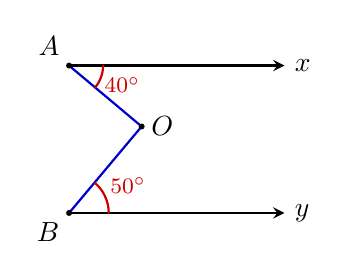
\begin{tikzpicture}[scale=0.72, line join=round, line cap=round, >=stealth]
    \coordinate (A) at (0,2.6);
    \coordinate (B) at (0,0);
    \draw[thick, ->] (A) -- ++(3.8,0) node[right] {$x$};
    \draw[thick, ->] (B) -- ++(3.8,0) node[right] {$y$};
    \path[name path=lineA] (A) -- ++(-40:4.2);
    \path[name path=lineB] (B) -- ++(50:4.2);
    \path [name intersections={of=lineA and lineB, by=O}];
    \draw[thick, blue!80!black] (A) -- (O) -- (B);
    \fill (A) circle (1.5pt) node[above left] {$A$};
    \fill (B) circle (1.5pt) node[below left] {$B$};
    \fill (O) circle (1.5pt) node[right] {$O$};
    \draw[red!80!black, thick] (A) ++(0.6,0) arc (0:-40:0.6);
    \path (A) ++(-20:1.0) node[red!80!black, font=\footnotesize] {$40^\circ$};
    \draw[red!80!black, thick] (B) ++(0.7,0) arc (0:50:0.7);
    \path (B) ++(25:1.15) node[red!80!black, font=\footnotesize] {$50^\circ$};
\end{tikzpicture}
\vspace{0.5mm}
&
\oGTKL
\\ \hline
\oBaiTap[12]{a)}{} &
\oBaiTap[12]{b)}{}
\\ \hline
\end{tabularx}

\newpage
% =============================================================================
% ========================= TOÁN 7 - TUẦN 05 - BUỔI 02: MÃ ĐỀ 102 =============
% ========================= MẶT TRƯỚC (TRANG 1/2) ==============================
% =============================================================================

\noindent
\begin{tabularx}{\linewidth}{|X|c|}
\hline
\textbf{PHIẾU KIỂM TRA ĐỊNH KỲ TOÁN 7 - TUẦN 05 - BUỔI 02} & \textbf{Mã đề: 102 - Trang 1/2} \\
\textit{Chủ đề: Tổng ôn tập Số hữu tỉ \& Hình học tính góc} & \textit{Thời gian: 45 phút} \\
\hline
\end{tabularx}

\vspace{0.8mm}

\noindent
\begin{tabularx}{\linewidth}{|X|}
\hline
\rule[-2mm]{0pt}{8mm}\textbf{Họ và tên học sinh:} \hfill \textbf{SĐT:} \makebox[4.5cm]{\dotfill} \\
\hline
\end{tabularx}

\vspace{0.8mm}

\noindent
\begin{tabularx}{\linewidth}{|p{3.2cm}|X|}
\hline
\centering\textbf{ĐIỂM SỐ} & \centering\textbf{LỜI NHẬN XÉT CỦA THẦY CÔ} \tabularnewline
\hline
\rule{0pt}{1.8cm} & \tabularnewline
\hline
\end{tabularx}

\vspace{1mm}

\noindent\textbf{\large PHẦN I. TRẮC NGHIỆM KHÁCH QUAN (2,5 điểm)} \hfill \textit{(Khoanh tròn đáp án đúng)}
\vspace{0.8mm}

\cauTN{1}{Làm tròn số thập phân $a = 15{,}728$ đến hàng phần mười ta được số:}{$15{,}73$}{$15{,}7$}{$15{,}8$}{$16{,}0$}

\cauTN{2}{Khẳng định nào sau đây là \textbf{đúng} về quy tắc lũy thừa?}{$x^3 \cdot x^4 = x^{12}$}{$(x^2)^3 = x^5$}{$x^6 : x^2 = x^4$ ($x \ne 0$)}{$\left(\dfrac{a}{b}\right)^2 = \dfrac{a}{b^2}$}

\cauTN{3}{Cho đẳng thức $x - \dfrac{2}{5} = -\dfrac{1}{3}$. Theo quy tắc chuyển vế thì $x$ bằng:}{$-\dfrac{1}{3} + \dfrac{2}{5}$}{$-\dfrac{1}{3} - \dfrac{2}{5}$}{$\dfrac{2}{5} - \left(-\dfrac{1}{3}\right)$}{$\dfrac{1}{3} + \dfrac{2}{5}$}

\cauTN{4}{Nếu đường thẳng $c$ cắt hai đường thẳng song song $m$ và $n$ thì hai góc so le trong:}{bù nhau}{phụ nhau}{bằng nhau}{kề bù}

\cauTN{5}{Cho hai đường thẳng phân biệt $m, n$ cùng vuông góc với đường thẳng $p$ thì:}{$m \parallel n$}{$m \perp n$}{$m$ cắt $n$}{$m \equiv n$}

\vspace{1mm}

\noindent\textbf{\large PHẦN II. TỰ LUẬN (7,5 điểm)}

\noindent\textbf{Câu 2 (2,5 điểm). Thực hiện phép tính (hợp lý nếu có thể):}
\vspace{0.5mm}

\noindent
\begin{tabularx}{\linewidth}{|X|X|}
\hline
\oBaiTap[8]{a)}{$\dfrac{2}{3} - \dfrac{3}{4} + \dfrac{5}{12}$} & 
\oBaiTap[8]{b)}{$\dfrac{9}{17} \cdot \left(-\dfrac{4}{9}\right) + \dfrac{9}{17} \cdot \left(-\dfrac{5}{9}\right)$} \\
\hline
\oBaiTap[8]{c)}{$\left(-\dfrac{1}{3}\right)^2 + \dfrac{5}{6} \cdot \left(-\dfrac{2}{5}\right) - \left(-\dfrac{2}{5}\right)^0$} & 
\oBaiTap[8]{d)}{$\dfrac{5}{6} - \left[\dfrac{1}{3} + \left(\dfrac{2}{5} - \dfrac{7}{10}\right)\right]$} \\
\hline
\end{tabularx}

\newpage
% =============================================================================
% ========================= TOÁN 7 - TUẦN 05 - BUỔI 02: MÃ ĐỀ 102 =============
% ========================= MẶT SAU (TRANG 2/2) ================================
% =============================================================================

\noindent
\begin{tabularx}{\linewidth}{|X|c|}
\hline
\textbf{PHẦN II. TỰ LUẬN (Tiếp theo) - TOÁN 7 TUẦN 05 BUỔI 02} & \textbf{Mã đề: 102 - Trang 2/2} \\
\hline
\end{tabularx}

\vspace{1mm}

\noindent\textbf{\large Câu 3 (2,5 điểm). Tìm số hữu tỉ $x$, biết:}
\vspace{0.5mm}

\noindent
\begin{tabularx}{\linewidth}{|X|X|}
\hline
\oBaiTap[7]{a)}{$x - \dfrac{2}{3} = \dfrac{5}{6}$} & 
\oBaiTap[7]{b)}{$\dfrac{2}{3}x + \dfrac{1}{4} = -\dfrac{5}{12}$} \\
\hline
\oBaiTap[7]{c)}{$\left(x + \dfrac{1}{3}\right)^2 = \dfrac{25}{36}$} & 
\oBaiTap[7]{d)}{$\left(x - \dfrac{3}{5}\right)\left(3x + \dfrac{1}{2}\right) = 0$} \\
\hline
\end{tabularx}

\vspace{1mm}

\noindent\textbf{\large Câu 4 (2,5 điểm).} Cho hình vẽ, biết $Ax \parallel By$, $\widehat{xAO} = 35^\circ$ và $\widehat{yBO} = 55^\circ$:\par\vspace{0.3mm}
\noindent\textbf{a) (1,25 điểm)} Kẻ tia $Oz \parallel Ax$ ($Oz$ nằm trong góc $\widehat{AOB}$). Chứng minh rằng $Oz \parallel By$.\par\vspace{0.2mm}
\noindent\textbf{b) (1,25 điểm)} Chỉ ra các cặp góc so le trong, từ đó tính số đo của góc $\widehat{AOB}$.\par\vspace{0.5mm}

\noindent
\begin{tabularx}{\linewidth}{|X|X|}
\hline
\vspace{0.5mm}
\centering
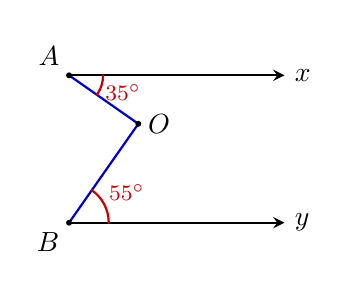
\begin{tikzpicture}[scale=0.72, line join=round, line cap=round, >=stealth]
    \coordinate (A) at (0,2.6);
    \coordinate (B) at (0,0);
    \draw[thick, ->] (A) -- ++(3.8,0) node[right] {$x$};
    \draw[thick, ->] (B) -- ++(3.8,0) node[right] {$y$};
    \path[name path=lineA] (A) -- ++(-35:4.2);
    \path[name path=lineB] (B) -- ++(55:4.2);
    \path [name intersections={of=lineA and lineB, by=O}];
    \draw[thick, blue!80!black] (A) -- (O) -- (B);
    \fill (A) circle (1.5pt) node[above left] {$A$};
    \fill (B) circle (1.5pt) node[below left] {$B$};
    \fill (O) circle (1.5pt) node[right] {$O$};
    \draw[red!80!black, thick] (A) ++(0.6,0) arc (0:-35:0.6);
    \path (A) ++(-17.5:1.0) node[red!80!black, font=\footnotesize] {$35^\circ$};
    \draw[red!80!black, thick] (B) ++(0.7,0) arc (0:55:0.7);
    \path (B) ++(27.5:1.15) node[red!80!black, font=\footnotesize] {$55^\circ$};
\end{tikzpicture}
\vspace{0.5mm}
&
\oGTKL
\\ \hline
\oBaiTap[12]{a)}{} &
\oBaiTap[12]{b)}{}
\\ \hline
\end{tabularx}

\newpage
% =============================================================================
% ========================= TOÁN 7 - TUẦN 05 - BUỔI 02: MÃ ĐỀ 103 =============
% ========================= MẶT TRƯỚC (TRANG 1/2) ==============================
% =============================================================================

\noindent
\begin{tabularx}{\linewidth}{|X|c|}
\hline
\textbf{PHIẾU KIỂM TRA ĐỊNH KỲ TOÁN 7 - TUẦN 05 - BUỔI 02} & \textbf{Mã đề: 103 - Trang 1/2} \\
\textit{Chủ đề: Tổng ôn tập Số hữu tỉ \& Hình học tính góc} & \textit{Thời gian: 45 phút} \\
\hline
\end{tabularx}

\vspace{0.8mm}

\noindent
\begin{tabularx}{\linewidth}{|X|}
\hline
\rule[-2mm]{0pt}{8mm}\textbf{Họ và tên học sinh:} \hfill \textbf{SĐT:} \makebox[4.5cm]{\dotfill} \\
\hline
\end{tabularx}

\vspace{0.8mm}

\noindent
\begin{tabularx}{\linewidth}{|p{3.2cm}|X|}
\hline
\centering\textbf{ĐIỂM SỐ} & \centering\textbf{LỜI NHẬN XÉT CỦA THẦY CÔ} \tabularnewline
\hline
\rule{0pt}{1.8cm} & \tabularnewline
\hline
\end{tabularx}

\vspace{1mm}

\noindent\textbf{\large PHẦN I. TRẮC NGHIỆM KHÁCH QUAN (2,5 điểm)} \hfill \textit{(Khoanh tròn đáp án đúng)}
\vspace{0.8mm}

\cauTN{1}{Làm tròn số $28{,}645$ đến hàng phần mười ta được số:}{$28{,}7$}{$28{,}65$}{$28{,}6$}{$29{,}0$}

\cauTN{2}{Kết quả của phép tính lũy thừa $\left(-\dfrac{2}{3}\right)^2$ là:}{$-\dfrac{4}{9}$}{$\dfrac{4}{9}$}{$\dfrac{4}{6}$}{$-\dfrac{4}{6}$}

\cauTN{3}{Cho đẳng thức $\dfrac{3}{5} - x = \dfrac{1}{2}$. Theo quy tắc chuyển vế thì $x$ bằng:}{$\dfrac{1}{2} - \dfrac{3}{5}$}{$\dfrac{1}{2} + \dfrac{3}{5}$}{$\dfrac{3}{5} - \dfrac{1}{2}$}{$-\dfrac{3}{5} - \dfrac{1}{2}$}

\cauTN{4}{Nếu một đường thẳng cắt hai đường thẳng song song thì hai góc đồng vị:}{bù nhau}{phụ nhau}{bằng nhau}{kề bù}

\cauTN{5}{Cho ba đường thẳng phân biệt $a, b, c$. Nếu $a \parallel c$ và $b \parallel c$ thì:}{$a \parallel b$}{$a \perp b$}{$a \equiv b$}{$a$ cắt $b$}

\vspace{1mm}

\noindent\textbf{\large PHẦN II. TỰ LUẬN (7,5 điểm)}

\noindent\textbf{Câu 2 (2,5 điểm). Thực hiện phép tính (hợp lý nếu có thể):}
\vspace{0.5mm}

\noindent
\begin{tabularx}{\linewidth}{|X|X|}
\hline
\oBaiTap[8]{a)}{$\dfrac{4}{7} - \dfrac{1}{2} + \dfrac{5}{14}$} & 
\oBaiTap[8]{b)}{$\dfrac{8}{13} \cdot \left(-\dfrac{2}{7}\right) + \dfrac{8}{13} \cdot \left(-\dfrac{5}{7}\right)$} \\
\hline
\oBaiTap[8]{c)}{$\left(-\dfrac{1}{2}\right)^3 + \dfrac{2}{3} \cdot \left(-\dfrac{3}{4}\right) + \left(\dfrac{1}{2}\right)^0$} & 
\oBaiTap[8]{d)}{$\dfrac{3}{4} - \left[\dfrac{1}{6} + \left(\dfrac{3}{5} - \dfrac{9}{10}\right)\right]$} \\
\hline
\end{tabularx}

\newpage
% =============================================================================
% ========================= TOÁN 7 - TUẦN 05 - BUỔI 02: MÃ ĐỀ 103 =============
% ========================= MẶT SAU (TRANG 2/2) ================================
% =============================================================================

\noindent
\begin{tabularx}{\linewidth}{|X|c|}
\hline
\textbf{PHẦN II. TỰ LUẬN (Tiếp theo) - TOÁN 7 TUẦN 05 BUỔI 02} & \textbf{Mã đề: 103 - Trang 2/2} \\
\hline
\end{tabularx}

\vspace{1mm}

\noindent\textbf{\large Câu 3 (2,5 điểm). Tìm số hữu tỉ $x$, biết:}
\vspace{0.5mm}

\noindent
\begin{tabularx}{\linewidth}{|X|X|}
\hline
\oBaiTap[7]{a)}{$\dfrac{3}{5} - x = \dfrac{1}{10}$} & 
\oBaiTap[7]{b)}{$\dfrac{4}{5}x - \dfrac{2}{3} = \dfrac{1}{3}$} \\
\hline
\oBaiTap[7]{c)}{$\left(x - \dfrac{2}{3}\right)^2 = \dfrac{1}{16}$} & 
\oBaiTap[7]{d)}{$\left(x + \dfrac{4}{7}\right)\left(2x - \dfrac{5}{3}\right) = 0$} \\
\hline
\end{tabularx}

\vspace{1mm}

\noindent\textbf{\large Câu 4 (2,5 điểm).} Cho hình vẽ, biết $Ax \parallel By$, $\widehat{xAO} = 45^\circ$ và $\widehat{yBO} = 65^\circ$:\par\vspace{0.3mm}
\noindent\textbf{a) (1,25 điểm)} Kẻ tia $Oz \parallel Ax$ ($Oz$ nằm trong góc $\widehat{AOB}$). Chứng minh rằng $Oz \parallel By$.\par\vspace{0.2mm}
\noindent\textbf{b) (1,25 điểm)} Chỉ ra các cặp góc so le trong, từ đó tính số đo của góc $\widehat{AOB}$.\par\vspace{0.5mm}

\noindent
\begin{tabularx}{\linewidth}{|X|X|}
\hline
\vspace{0.5mm}
\centering
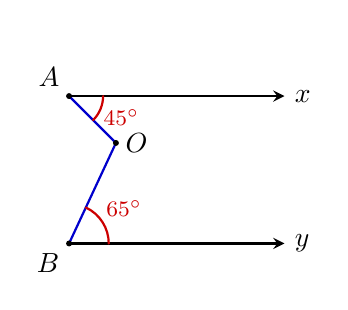
\begin{tikzpicture}[scale=0.72, line join=round, line cap=round, >=stealth]
    \coordinate (A) at (0,2.6);
    \coordinate (B) at (0,0);
    \draw[thick, ->] (A) -- ++(3.8,0) node[right] {$x$};
    \draw[thick, ->] (B) -- ++(3.8,0) node[right] {$y$};
    \path[name path=lineA] (A) -- ++(-45:4.2);
    \path[name path=lineB] (B) -- ++(65:4.2);
    \path [name intersections={of=lineA and lineB, by=O}];
    \draw[thick, blue!80!black] (A) -- (O) -- (B);
    \fill (A) circle (1.5pt) node[above left] {$A$};
    \fill (B) circle (1.5pt) node[below left] {$B$};
    \fill (O) circle (1.5pt) node[right] {$O$};
    \draw[red!80!black, thick] (A) ++(0.6,0) arc (0:-45:0.6);
    \path (A) ++(-22.5:1.0) node[red!80!black, font=\footnotesize] {$45^\circ$};
    \draw[red!80!black, thick] (B) ++(0.7,0) arc (0:65:0.7);
    \path (B) ++(32.5:1.15) node[red!80!black, font=\footnotesize] {$65^\circ$};
\end{tikzpicture}
\vspace{0.5mm}
&
\oGTKL
\\ \hline
\oBaiTap[12]{a)}{} &
\oBaiTap[12]{b)}{}
\\ \hline
\end{tabularx}

\newpage
% =============================================================================
% ========================= TOÁN 7 - TUẦN 05 - BUỔI 02: MÃ ĐỀ 104 =============
% ========================= MẶT TRƯỚC (TRANG 1/2) ==============================
% =============================================================================

\noindent
\begin{tabularx}{\linewidth}{|X|c|}
\hline
\textbf{PHIẾU KIỂM TRA ĐỊNH KỲ TOÁN 7 - TUẦN 05 - BUỔI 02} & \textbf{Mã đề: 104 - Trang 1/2} \\
\textit{Chủ đề: Tổng ôn tập Số hữu tỉ \& Hình học tính góc} & \textit{Thời gian: 45 phút} \\
\hline
\end{tabularx}

\vspace{0.8mm}

\noindent
\begin{tabularx}{\linewidth}{|X|}
\hline
\rule[-2mm]{0pt}{8mm}\textbf{Họ và tên học sinh:} \hfill \textbf{SĐT:} \makebox[4.5cm]{\dotfill} \\
\hline
\end{tabularx}

\vspace{0.8mm}

\noindent
\begin{tabularx}{\linewidth}{|p{3.2cm}|X|}
\hline
\centering\textbf{ĐIỂM SỐ} & \centering\textbf{LỜI NHẬN XÉT CỦA THẦY CÔ} \tabularnewline
\hline
\rule{0pt}{1.8cm} & \tabularnewline
\hline
\end{tabularx}

\vspace{1mm}

\noindent\textbf{\large PHẦN I. TRẮC NGHIỆM KHÁCH QUAN (2,5 điểm)} \hfill \textit{(Khoanh tròn đáp án đúng)}
\vspace{0.8mm}

\cauTN{1}{Làm tròn số $\sqrt{10} \approx 3{,}16227...$ đến hàng phần trăm ta được số:}{$3{,}16$}{$3{,}17$}{$3{,}162$}{$3{,}2$}

\cauTN{2}{Giá trị của biểu thức lũy thừa $\left(\dfrac{2}{3}\right)^3 : \left(\dfrac{2}{3}\right)^2$ là:}{$\dfrac{4}{9}$}{$\dfrac{8}{27}$}{$\dfrac{2}{3}$}{$1$}

\cauTN{3}{Cho đẳng thức $x + \dfrac{1}{4} = -\dfrac{2}{3}$. Theo quy tắc chuyển vế thì $x$ bằng:}{$-\dfrac{2}{3} - \dfrac{1}{4}$}{$-\dfrac{2}{3} + \dfrac{1}{4}$}{$\dfrac{1}{4} - \left(-\dfrac{2}{3}\right)$}{$\dfrac{2}{3} - \dfrac{1}{4}$}

\cauTN{4}{Nếu một đường thẳng cắt hai đường thẳng song song thì hai góc đồng vị:}{bù nhau}{bằng nhau}{phụ nhau}{kề bù}

\cauTN{5}{Cho hai đường thẳng phân biệt $x, y$ cùng song song với đường thẳng $z$ thì:}{$x \perp y$}{$x$ cắt $y$}{$x \parallel y$}{$x \equiv y$}

\vspace{1mm}

\noindent\textbf{\large PHẦN II. TỰ LUẬN (7,5 điểm)}

\noindent\textbf{Câu 2 (2,5 điểm). Thực hiện phép tính (hợp lý nếu có thể):}
\vspace{0.5mm}

\noindent
\begin{tabularx}{\linewidth}{|X|X|}
\hline
\oBaiTap[8]{a)}{$\dfrac{5}{8} - \dfrac{3}{4} + \dfrac{7}{16}$} & 
\oBaiTap[8]{b)}{$\dfrac{6}{19} \cdot \left(-\dfrac{5}{11}\right) + \dfrac{6}{19} \cdot \left(-\dfrac{6}{11}\right)$} \\
\hline
\oBaiTap[8]{c)}{$\left(-\dfrac{2}{3}\right)^2 + \dfrac{1}{2} \cdot \left(-\dfrac{4}{3}\right) - \left(-\dfrac{3}{7}\right)^0$} & 
\oBaiTap[8]{d)}{$\dfrac{7}{10} - \left[\dfrac{1}{4} + \left(\dfrac{5}{6} - \dfrac{11}{12}\right)\right]$} \\
\hline
\end{tabularx}

\newpage
% =============================================================================
% ========================= TOÁN 7 - TUẦN 05 - BUỔI 02: MÃ ĐỀ 104 =============
% ========================= MẶT SAU (TRANG 2/2) ================================
% =============================================================================

\noindent
\begin{tabularx}{\linewidth}{|X|c|}
\hline
\textbf{PHẦN II. TỰ LUẬN (Tiếp theo) - TOÁN 7 TUẦN 05 BUỔI 02} & \textbf{Mã đề: 104 - Trang 2/2} \\
\hline
\end{tabularx}

\vspace{1mm}

\noindent\textbf{\large Câu 3 (2,5 điểm). Tìm số hữu tỉ $x$, biết:}
\vspace{0.5mm}

\noindent
\begin{tabularx}{\linewidth}{|X|X|}
\hline
\oBaiTap[7]{a)}{$\dfrac{5}{6} - x = \dfrac{1}{4}$} & 
\oBaiTap[7]{b)}{$\dfrac{5}{6}x + \dfrac{1}{3} = -\dfrac{1}{2}$} \\
\hline
\oBaiTap[7]{c)}{$\left(x + \dfrac{1}{4}\right)^2 = \dfrac{9}{25}$} & 
\oBaiTap[7]{d)}{$\left(x - \dfrac{5}{6}\right)\left(4x + \dfrac{2}{3}\right) = 0$} \\
\hline
\end{tabularx}

\vspace{1mm}

\noindent\textbf{\large Câu 4 (2,5 điểm).} Cho hình vẽ, biết $Ax \parallel By$, $\widehat{xAO} = 50^\circ$ và $\widehat{yBO} = 60^\circ$:\par\vspace{0.3mm}
\noindent\textbf{a) (1,25 điểm)} Kẻ tia $Oz \parallel Ax$ ($Oz$ nằm trong góc $\widehat{AOB}$). Chứng minh rằng $Oz \parallel By$.\par\vspace{0.2mm}
\noindent\textbf{b) (1,25 điểm)} Chỉ ra các cặp góc so le trong, từ đó tính số đo của góc $\widehat{AOB}$.\par\vspace{0.5mm}

\noindent
\begin{tabularx}{\linewidth}{|X|X|}
\hline
\vspace{0.5mm}
\centering
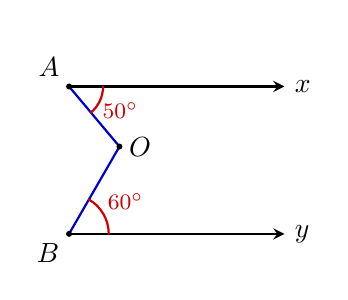
\begin{tikzpicture}[scale=0.72, line join=round, line cap=round, >=stealth]
    \coordinate (A) at (0,2.6);
    \coordinate (B) at (0,0);
    \draw[thick, ->] (A) -- ++(3.8,0) node[right] {$x$};
    \draw[thick, ->] (B) -- ++(3.8,0) node[right] {$y$};
    \path[name path=lineA] (A) -- ++(-50:4.2);
    \path[name path=lineB] (B) -- ++(60:4.2);
    \path [name intersections={of=lineA and lineB, by=O}];
    \draw[thick, blue!80!black] (A) -- (O) -- (B);
    \fill (A) circle (1.5pt) node[above left] {$A$};
    \fill (B) circle (1.5pt) node[below left] {$B$};
    \fill (O) circle (1.5pt) node[right] {$O$};
    \draw[red!80!black, thick] (A) ++(0.6,0) arc (0:-50:0.6);
    \path (A) ++(-25:1.0) node[red!80!black, font=\footnotesize] {$50^\circ$};
    \draw[red!80!black, thick] (B) ++(0.7,0) arc (0:60:0.7);
    \path (B) ++(30:1.15) node[red!80!black, font=\footnotesize] {$60^\circ$};
\end{tikzpicture}
\vspace{0.5mm}
&
\oGTKL
\\ \hline
\oBaiTap[12]{a)}{} &
\oBaiTap[12]{b)}{}
\\ \hline
\end{tabularx}

\end{document}
